\documentclass[a4paper,12pt,ngerman]{scrartcl}

% Language
\usepackage{polyglossia}
\setmainlanguage{german}

% Grafiken
\usepackage{graphicx}

% Make \today print in format "NN<st|nd|rd|th> MM YYYY"
\usepackage{isodate}
\origdate

\linespread{1.15}

% Titel anders formatieren mit: Command, Format, Label, Sep, Before-Code
\usepackage{titlesec}
\titleformat{\section}{\sffamily\Large\bfseries}{}{0pt}{}
\titleformat{\subsection}{\sffamily\large\bfseries}{}{0pt}{}

% Own pagestyle (header and footer)
\usepackage{fancyhdr}
\fancyhf{} % Clear header and footer content
\fancyhead[L]{{\small \textsf{WS 14/15, Informationsvisualisierung}}}
\fancyhead[C]{{\small \textsf{Übung 5}}}
\fancyhead[R]{{\small \textsf{\today}}}
\fancyfoot[C]{\thepage}

% Text in quotes
% Usage: \enquote{To be or not to be.}
\usepackage{csquotes}

% Subliminal refinements towards typographical perfection
\usepackage{microtype}

% Footnotes in section
\usepackage[stable]{footmisc}

% Better refs with \cref{}
\usepackage[capitalize,noabbrev]{cleveref}

% Borders
\usepackage[paper=a4paper,left=20mm,right=20mm,top=30mm,bottom=30mm]{geometry}

\usepackage{placeins}

\begin{document}
\pagestyle{fancy} % Activate own pagestyle

\section{Aufgabe 5.1 | Word Clouds}
Text...
%\begin{figure}[ht]
%    \centering
%    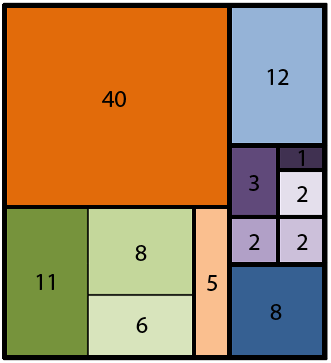
\includegraphics[height=10cm]{includes/SquarifiedTreemaps2}
%    \caption{Squarified Treemap - absteigende Reihenfolge}
%    \label{fig:squarifiedTreemap2}
%\end{figure}

\section{Aufgabe 5.2 | DNA-Sequenzen}
Text...
\end{document}
